\documentclass{article}
\usepackage{longtable}
\usepackage{xcolor}
\usepackage{enumitem}
\usepackage{geometry}
\usepackage{float}
\usepackage{url}
\usepackage{graphicx}
\usepackage{amsmath}
\usepackage{listings}
\usepackage{microtype}
\usepackage{hyperref}
\usepackage{adjustbox}

\newcommand\ytl[2]{
    \parbox[b]{12em}{\hfill{\color{cyan}\bfseries\sffamily #1}~$\cdots\cdots$~}\makebox[0pt][c]{$\bullet$}\vrule\quad
    \parbox[c]{10cm}{\vspace{6pt}\color[RGB]{20, 20, 90}\raggedright\sffamily #2\par}
    \\[-2pt]
}

\title{Creating Software for Value at Risk}
\author{Benjamin Shearlock}

\begin{document}
\raggedright

\begin{titlepage}
  \begin{center}
    \vspace*{1cm}
    {\LARGE \textbf{Creating Software for Value at Risk} \par} 
    \vspace{1.5cm}
    {\Large \textit{Interim Report} \par}
    \vspace{0.5cm}
    {\Large BSc Final Year Project \par}
    \vspace{2cm}
    {\large \textbf{Author} \par}
    {\large Benjamin Shearlock \par}
    \vspace{2cm}
    {\large \textbf{Supervisor} \par}
    {\large Dr. Volodya Vovk \par}
    \vfill
    {\large Department of Computer Science \par}
    {\large Royal Holloway, University of London \par}
  \end{center}
\end{titlepage}

\setlength{\parindent}{0pt}

\section*{Declaration}
I have read and understood the Universities regulations on plagiarism and I hereby declare that all work submitted in this project is my own, except where explicitly stated otherwise, such as the references that have been cited. \\

\begin{itemize}
  \item Word Count: 12,669
  \item Name: Benjamin Charles Shearlock
  \item Submission Date: 08/12/2023
  \item Youtube Video showcasing Term 1 main program: \url{https://youtu.be/2GIWug_IESI}
  \item All other programs included within my PROJECT Git repository are simple python programs that can just be ran normally, these mainly being found within the ``Command Line VaR Programs'' folder. The GUI program has been compiled into a .exe file within the main directory, called “Initial Design Test.exe”, it will open up a terminal when ran but please ignore it, it should work perfectly otherwise. The code for it is within the ``Kivy'' folder, that has other kivy tests inside it as well. It is all in the branch ``Master'', as I was having issues with my ``Main'' branch. If viewing from the Zip submitted, it should not matter about the branch.
  \item Git Repository: \url{https://gitlab.cim.rhul.ac.uk/zjac018/PROJECT/-/tree/master?ref_type=heads}

  % \item Signature: \includegraphics[scale=0.1]{Signature.png}
\end{itemize}

\newpage

\tableofcontents

\newpage

\section{Abstract}
In the realm of financial risk management, understanding and evaluating the level of risk associated with any investment or portfolio is of extremely high importance. Perhaps the most universally regarded metric used for this purpose is Value at Risk (VaR). VaR provides a quantitative estimate of the potential losses that a portfolio may incur over a certain period of time (specified time horizon) at a given confidence level. \\\vspace{0.3cm}

Original widespread use of VaR came about in the early 1990s, the concept first being introduced by J.P. Morgan in 1994, since it helped provide an estimate of the maximum loss an investor is willing to accept for any given investment. Its historical roots can be traced back to the financial industry's increasing need for a standardized and comprehensive measure of risk following the 1987 stock market crash, so they sought a comprehensive way to assess risk in complex portfolios [\ref{ref3}]. \\

Mathematically, VaR is expressed as follows:
\begin{equation}
VaR(N, X) = -\text{Percentile}(L, 1 - X)
\end{equation}
Where:
\begin{align*}
N & : \text{Time horizon (in days)} \\
X & : \text{Confidence level (in percentage)} \\
L & : \text{Loss distribution over } N \text{ days}
\end{align*}

This formula captures the loss at the \((100-X)\)th percentile of the loss distribution over the specified time horizon [\ref{ref6}]. \\\vspace{0.3cm}

VaR can be mathematically computed through various methods, each with its own strengths and limitations. The most common approaches include the historical simulation method, parametric method, model building method and Monte Carlo simulation [\ref{ref1}], to list a few. For historical simulation, past data is used to estimate future risk by examining the historical returns of an asset or portfolio, while model building employs mathematical models to predict portfolio performance. The choice of algorithm depends on data availability, computational resources, and specific requirements.\\\vspace{0.3cm}

To implement VaR calculations, various pieces of software are essential. In this project, I will be utilising Visual Studio Code (VSCode) as the integrated development environment (IDE) and Python for its rich ecosystem of libraries. Python libraries like NumPy, Matplotlib, and Kivy will be invaluable for data manipulation, visualisation, and user interface design [\ref{ref9}].\\\vspace{0.3cm}

My inaugural proof of concept program will be created to visually demonstrate VaR calculations for  two initial methods, these being historical simulation and model building techniques to estimate VaR for a sample portfolio. Historical simulation would involve collecting historical data and computing VaR based on past performance (can involve acquiring stock data through an API), while model building would use a predefined model to forecast future losses. Visualisation tools like Matplotlib can help in presenting the results graphically, enabling me to generate informative charts and graphs. NumPy will facilitate data manipulation and efficient mathematical operations [\ref{ref10}]. Additionally, Kivy, a Python framework for developing multi-touch applications, will be used to create the interfaces for the visual representation of VaR, as well as giving it the option to possibly be viewed on other devices.\\\vspace{0.3cm}

Later on into the project, if there is enough time, I think it may be worth exploring some more advanced topics like the variance-covariance of returns, specifically employing GARCH (Generalized Autoregressive Conditional Heteroscedasticity) models. GARCH models provide a more nuanced understanding of volatility and can enhance the accuracy of VaR estimates [\ref{ref6}].\\\vspace{0.3cm}

The objective of my project is to gain a deeper understanding of VaR, develop a functional program to calculate and visualise it, and potentially extend the research to incorporate more advanced risk management techniques if possible. This project is a stepping stone towards a deeper understanding of the risk side of finances and will contribute to enhancing the knowledge and skills necessary for effective financial decision-making, since this is not a topic that I have delved much into before, but I have aways been very interested in learning more about it. This gives me a fantastic opportunity to learn about the financial sector, as well as create something that is applicable and useful to real life. \\


% \section{Specification}

\newpage
\section{Chapter 1 - Introduction}

\subsection{What is VaR?}

Value at Risk (VaR) is a statistical value used to quantify the level of financial risk within a portfolio of stocks/derivatives over a specified time horizon. It estimates the maximum potential loss that an investment portfolio could incur with a given probability, known as the confidence level, under normal market conditions. The VaR metric is typically expressed in monetary terms and is often used to assess the risk of a portfolio of financial instruments. From a banks perspective, they would say:
\begin{quote}
  ``With \textbf{X\% confidence (1-X\% Risk Level)}, we expect to not lose more than \textbf{V} over the next \textbf{N day(s)} on our entire \textbf{portfolio} of derivatives, worth \textbf{Z}'' - [\ref{ref4}]

\end{quote}

Where:
\begin{align*}
  \textbf{X} & : \text{Confidence Level} \\
  \textbf{V} & : \text{Value at Risk} \\
  \textbf{N} & : \text{Time Horizon} \\
  \textbf{Z} & : \text{Portfolio Value}
\end{align*}

This is incredibly useful as it allows for a simple and easy to understand metric to be used to assess the risk of a portfolio, which is extremely important in the financial sector, taking all the underlying complexities of any form of portfolio and being able to conform its financial risk into a single, universally used, number. \\\vspace{0.3cm}

To include actual numbers, to easier explain how it would look, a bank would say:
\begin{quote}
  ``With \textbf{95\%} confidence (\textbf{5\%} Risk Level), we expect to not lose more than \textbf{£3,000,000} over the next \textbf{1 day} on our entire portfolio of derivatives, worth \textbf{£100,000,000}''
\end{quote}

This is essential to help financial institutions understand the level of risk associated with their portfolios, as well as being able to compare the risk of different portfolios, which is why it is such a widely used metric in the financial sector, limiting the level of risk that a person/organisation is exposed to.\\\vspace{0.3cm}

The concept of VaR has its roots in the late 20th century, gaining prominence in the finance industry during the 1990s. It emerged from the need for more sophisticated risk management tools in the wake of financial market liberalisation and the increasing complexity of financial instruments. The widespread adoption of VaR was catalysed by the 1998 financial crisis, where it played a significant role in risk assessment and regulatory frameworks.\\\vspace{0.3cm}


VaR is significant for several reasons:
\begin{itemize}
    \item \textbf{Risk Measurement:} VaR provides a quantitative measure of potential losses in a portfolio.
    \item \textbf{Decision Making:} VaR aids financial managers in making informed decisions about risk tolerance and capital allocation.
    \item \textbf{Market Risk Management:} VaR is used to monitor and mitigate market risks, contributing to the overall stability of financial systems.
\end{itemize}

VaR has become a cornerstone in risk management for global financial markets. It is used by banks, investment firms, asset managers, and corporates to measure and control the level of risk exposure in their financial portfolios. VaR's adoption is partly driven by regulatory requirements, such as Basel Accords, which mandate financial institutions to calculate and maintain adequate capital reserves based on their risk exposure.[\ref{ref12}]\\\vspace{0.3cm} 


Developing software for VaR calculation offers numerous advantages:
\begin{itemize}
    \item \textbf{Accessibility:} It establishes a widespread access to sophisticated risk management tools.
    \item \textbf{Efficiency:} Automated VaR calculations save time and reduce the potential for human error.
    \item \textbf{Customization:} Software can be tailored to specific needs and types of portfolios.
    \item \textbf{Real-Time Analysis:} It enables rapid and up-to-date risk assessments.
\end{itemize}

VaR has become an essential tool in modern financial risk management. The development of software for VaR calculations aligns with the need for efficient, accurate, and accessible risk management tools in today's fast-paced financial markets. This is what I want to help contribute to within this project.\\

\subsection{Aims and Goals}
My aims and goals for this project are as follows:

\begin{enumerate}
    \item \textbf{Comprehensive Understanding of VaR:} To touch on VaR's theoretical underpinnings and why it has such a pivotal role in modern financial risk management. This includes commenting on its applications across different financial groups, market conditions, and regulatory environments.
    
    \item \textbf{Methodological Exploration:} To investigate various computational methods for calculating VaR, including historical simulation, model building (variance-covariance) approach, and Monte Carlo Simulation, assessing their efficacy in different market scenarios. This will first be explored through command line programs, then later on through a GUI\@.
    
    \item \textbf{Technical Implementation:} Development of a comprehensive program for calculating and presenting VaR. This entails creating a user-friendly interface, ensuring accurate and efficient computation, and integrating various methods of VaR calculation to provide a comprehensive tool.
    
    \item \textbf{Application in Diverse Financial Contexts:} To ensure the software's adaptability and applicability in different financial settings. This includes testing the software with various data sets, portfolio types, and market conditions, aiming to make it a versatile tool for different financial entities.
    
    \item \textbf{Industry Standard Tool Development:} Creating a software application that not only performs standard VaR calculations but also offers other stock-oriented features, such as advanced data visualisation. The goal is to make the tool align with industry standards, ensuring it is suitable for professional financial risk management and has been developed whilst adhering to to industry principles in regard to software engineering.
\end{enumerate}

The ambition of this thesis is to present a thorough understanding of VaR, culminating in the development of a robust, adaptable, and industry-relevant tool for financial risk assessment. It aims to be acceptable as an industry standard tool, 
  
\subsection{Milestone Plan}
Due to unfortunate circumstances, I had rough delays to the start of this Project as well as inconsistent health concerns, but that should not effect my overall final deliverable. In the first term, I want to research and create a working program to compute Value at Risk for small portfolios, that has a serviceable GUI that can be expanded on later. I will also make sure to have amply researched about back-testing and how to incorporate it into my program in some capacity. For the second term, I will research and implement applying Value at Risk for a portfolio of derivatives, as well as looking into using the Monte Carlo simulation and allowing for the computation of all this with as many stocks as necessary. I will finalise the GUI and plan to look into completing some of the extensions provided for the project, this will depend on the overall developmental scope of the project at the time, but these are the options I would be willing to explore:

\begin{itemize}
  \item \textbf{Computing Conditional VaR (Expected Shortfall):}  Beyond the standard VaR metric, exploring Conditional VaR could be considered to provide a more comprehensive risk assessment, as it accounts for the severity of losses in the tail of the distribution.

  \item \textbf{Parameter Selection for EWMA and GARCH(1,1) Models:} A detailed analysis of parameter selection for the Exponentially Weighted Moving Average and GARCH(1,1) models could be explored. The choice of parameters greatly influences model performance, and overall it would enhance the robustness of the risk assessment.
  
  \item \textbf{Empirical Study of Approaches to Historical Simulation for n-day VaR:} A comparative empirical study could be undertaken to examine different approaches to extending historical simulation from 1-day to n-day VaR, which can provide deeper insights into the performance of the methods.
  
  \item \textbf{Complementing Back-Testing by Stress Testing:} The robustness of the VaR model could be assessed not only through back-testing but also by applying stress testing techniques, allowing for the evaluation of the model's performance under extreme market conditions.
  
  \item \textbf{Computing Monetary Measures of Risk Different from VaR:} Other monetary risk metrics, which could complement or provide alternatives to VaR, such as Tail Value at Risk, could be considered to present a more complete picture of the risk landscape and enhance the risk management process.
\end{itemize}

\newpage
The project's milestones have been structured to ensure a systematic and efficient approach to the development of the Value at Risk software. This plan is divided into distinct phases, each with specific objectives and deliverables.

  \begin{enumerate}
    \item \textbf{Initial Research and Planning (Completed):} This phase involved a thorough investigation into the concept of Value at Risk, its calculation methods, and the requirements for the software development.
    \item \textbf{Software Design and Development (Ongoing):} Currently, the focus is on designing the software and developing the core functionalities of the VaR calculation tool. This includes building the initial graphical user interface and implementing various VaR models into it.
    \item \textbf{Expanded GUI, Testing and Refinement:} After the development phase, there will be a complete redesign/refinement of the Graphical Interface, followed by rigorous testing that will be conducted to ensure the accuracy and reliability of the software. This phase will also involve refining the user interface and the overall user experience.
    \item \textbf{Final Evaluation and Documentation:} The final phase involves a comprehensive evaluation of the software against the project's objectives and preparing detailed documentation as well as informational videos.
  \end{enumerate}

  \subsubsection{Timescale \& Timeline}
  The entire project is structured over two academic terms, allowing ample time for each phase while ensuring a steady progression towards the project's completion. This timescale is designed to balance the initial development and subsequent refinement and testing phases effectively, ensuring that each aspect of the software is given due attention.\\\vspace{0.3cm}

  Concurrent with the development, ongoing documentation is a critical aspect of this project. Documenting the process as it unfolds serves multiple purposes: it ensures a clear record of the development process and aids in identifying and resolving issues more efficiently. This approach to documentation not only enhances the quality and maintainability of the software but also ensures that the project's progress is well-documented and aligns with the overall objectives and milestones.
% \subsubsection{Timeline}

\vspace{-2\baselineskip}
\begin{table}[H]
  \centering
  \color{black}
  \begin{longtable}{p{1\linewidth}}
    \endfirsthead
    \endhead
    \hspace*{\dimexpr\linewidth-0.721\linewidth}\rule{0.7\linewidth}{0.4pt}
    \ytl{Weeks 1--3}{
      \textbf{Project Research}
      \vspace{8pt}
      \begin{itemize}
          \item Research the fundamentals of Value at Risk (VaR)
          \item Research best coding language to use (Python)
          \item Familiarize myself with LaTeX and prepare IDE \& Git for Project specified use
      \end{itemize}
    } \vskip-19pt\hspace*{\dimexpr\linewidth-0.721\linewidth}\rule{0.7\linewidth}{0.4pt}
    \ytl{Week 4}{
      \textbf{Finalize Plan and Start Coding}
      \begin{itemize}
          \item Complete Project Plan
          \item Continue researching VaR and Python
          \item Begin project coding
      \end{itemize}
    } \vskip-19pt\hspace*{\dimexpr\linewidth-0.721\linewidth}\rule{0.7\linewidth}{0.4pt}
    \ytl{Week 5--7}{
      \textbf{Coding and Data Preparation}      
      \begin{itemize}
          \item Continue to work on the VaR program (No GUI)
          \item Start collecting and organizing sample data for small portfolios so it can be used by the program
          \item Finalizing understanding of the two computational methods needed, this being model-building and historical simulation
      \end{itemize}
    } \vskip-19pt\hspace*{\dimexpr\linewidth-0.721\linewidth}\rule{0.7\linewidth}{0.4pt}
    \ytl{Week 8}{
      \textbf{Back-Testing Research \& Implementation}      
      \begin{itemize}
          \item Investigate methods and techniques for VaR back-testing
          \item Start integrating back-testing into the project
      \end{itemize}
    } \vskip-19pt\hspace*{\dimexpr\linewidth-0.721\linewidth}\rule{0.7\linewidth}{0.4pt}
    \ytl{Week 9--10}{
      \textbf{GUI Development}      
      \begin{itemize}
          \item Initiate the development of the GUI
          \item Ensure the GUI is robust for its current task as well as expandable for future enhancements
      \end{itemize}
    } \vskip-19pt\hspace*{\dimexpr\linewidth-0.721\linewidth}\rule{0.7\linewidth}{0.4pt}
    \ytl{Week 11}{
      \textbf{Interim Report and Presentation Preparation}      
      \begin{itemize}
          \item Fine-tune programs and report so they are at a satisfactory level, will also allow for easier preparation for the interim presentation 
          \item Prepare for the interim presentation 
      \end{itemize}
    } \vskip-19pt\hspace*{\dimexpr\linewidth-0.721\linewidth}\rule{0.7\linewidth}{0.4pt}
  \end{longtable}
\end{table}

\vspace{-2\baselineskip}
\begin{table}[H]
  \centering
  \color{black}
  \begin{longtable}{p{1\linewidth}}
    \endfirsthead
    \endhead
    \vskip-19pt\hspace*{\dimexpr\linewidth-0.721\linewidth}\rule{0.7\linewidth}{0.4pt}
    \ytl{Weeks 1--2}{
      \textbf{Reflection and Research}
      \vspace{8pt}
      \begin{itemize}
          \item Spend time to reflect on the progress of the project so far, make any changes that I think are warranted after having the winter break time to think about
          \item Research the Monte Carlo simulation method for VaR, as well as how I could start implementing derivatives as portfolios into the project
      \end{itemize}
    } \vskip-19pt\hspace*{\dimexpr\linewidth-0.721\linewidth}\rule{0.7\linewidth}{0.4pt} 
    \ytl{Week 3--4}{
      \textbf{Start Implementing New Features}
  
      \begin{itemize}
          \item Start implementing the Monte Carlo simulation method and continue derivative implementation
          \item Start researching Eigen \& Cholesky decomposition to allow for however many stocks are needed within a portfolio
      \end{itemize}
    } \vskip-19pt\hspace*{\dimexpr\linewidth-0.721\linewidth}\rule{0.7\linewidth}{0.4pt} 
    \ytl{Week 5--7}{
      \textbf{GUI Finalisation}
      \begin{itemize}
          \item Decide on the final visual product I want to represent with the GUI and start implementing it (if progress on this needs to continue into the next period, then it will be done so)
          \item Set the program up to work portably/allowing it to work on mobile OS's as well as different desktop OS's
      \end{itemize}
    } \vskip-19pt\hspace*{\dimexpr\linewidth-0.721\linewidth}\rule{0.7\linewidth}{0.4pt} 
    \ytl{Week 8--9}{
      \textbf{Extend Project Scope (if time permits)}
      \begin{itemize}
          \item Explore additional features or enhancements for the project, possibly decided upon at the start of Term 2
          \item Implement as many as can be appropriately managed, with all additional time spent within this period being used to ensure the project is at its most refined state
      \end{itemize}
    } \vskip-19pt\hspace*{\dimexpr\linewidth-0.721\linewidth}\rule{0.7\linewidth}{0.4pt} 
    \ytl{Week 10--11}{
      \textbf{Perfect Final Report}
      \begin{itemize}
          \item Make sure the program has been achieved to the best of its ability
          \item Finalise and perfect the final report
      \end{itemize}
    } \vskip-19pt\hspace*{\dimexpr\linewidth-0.721\linewidth}\rule{0.7\linewidth}{0.4pt} 
  \end{longtable}
\end{table}

\section{Chapter 2 --- Understanding VaR}

\subsection{Historical Simulation}

Historical Simulation is a method of estimating Value at Risk (VaR). It relies on historical market data to predict future risks, making it a straightforward yet powerful method for calculating VaR. The process of computing VaR through Historical Simulation involves several steps, as outlined below:

\begin{enumerate}
    \item \textbf{Data Collection:} Historical price data of the asset is collected for a specified time period. This can be done using an API or through a CSV file.
    \item \textbf{Calculate Percentage Differences:} The daily returns are calculated, this being done by comparing the closing price of the current day to the closing price of the previous day by dividing one by the other, the taking away 1. This is done for each day in the data set.
    \item \textbf{Sort Returns:} The calculated returns are sorted in ascending order.
    \item \textbf{Determine the VaR Threshold:} A percentile is chosen based on the confidence level (e.g. 95\%). This is used to work out 100\% - X percentile (e.g. 5th), this being the risk level of the portfolio and X being the confidence level. This is the VaR threshold.
    \item \textbf{VaR Estimation:} The Value at Risk is estimated as the value at the chosen percentile. For example, if you have 500 days of data, the 5th percentile would be the 25th value in the sorted list of returns, then multiplied by the portfolio value, simulating the worst percentage decrease that your portfolio could encounter based on the last Z days of data.
    \item \textbf{Correct Negative Number:} Since it takes the 5th percentile, it will be a negative percentage difference multiplied by the portfolio, since we need to represent VaR as a positive value of potential loss, it is multiplied by -1 to make it positive.
\end{enumerate}

As you can see, it takes a very literal approach, assuming that, since you've got all this historical data, then it is likely that the future will be similar to the data of the past. It is an empirical method, meaning it is based on historical data, and as such is a simple and easy to understand, but it does have its limitations, such as the fact that it does not take into account any changes in the market, such as a financial crisis, which could have a huge impact on the market.\\\vspace{0.3cm}

\begin{figure}[h]
  \centering
  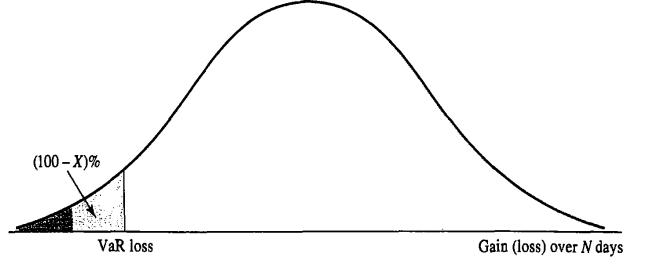
\includegraphics[width=0.5\textwidth]{Images/Image 1.png}
  \caption{The Value at Risk (VaR) is calculated from the probability distribution of the variations in the portfolio's value, where gains are represented as positive values and losses as negative. The confidence level for this calculation is set at X\%.[\ref{ref4}]}
  \label{VaR Distribution Curve}
\end{figure}

Refer to Figure~\ref{VaR Distribution Curve}, it expresses that:  
\begin{itemize}
  \item The bell-shaped curve represents the probability distribution of gains and losses for the asset or portfolio over the specified period.
  
  \item The left tail of the distribution marks the area of losses, where we can observe the VaR loss at a specific confidence level, say \( (100 - X)\% \). This tail area signifies the worst losses incurred in the historical period.
  
  \item The point where the left tail cuts the horizontal axis (gain/loss over N days) corresponds to the VaR at the chosen confidence level. For example, if \( X \) is 95, then the VaR would represent the maximum expected loss over the N days period that only 5\% of the time is expected to be exceeded.
  
  \item The graph assumes that the past can be a predictor of future risk, thus the frequency and magnitude of historical losses are directly used to estimate the VaR.
\end{itemize}

In the future, I could also use extreme value theory (EVT) to smooth our the distribution, which would allow for a more accurate estimation of the VaR, as it would allow for a better estimation of the tail of the distribution, which is where the worst losses are.[\ref{ref6}]\\\vspace{0.3cm}

\subsection{Model Building (Variance-Covariance)}

The Variance-Covariance method, used in this analysis for Value at Risk (VaR) calculation, is based on the assumption of normally distributed market returns. The key steps in the model are as follows:

\begin{enumerate}
    \item \textbf{Data Collection:} Historical price data of the asset is collected for a specified time period once again. This can be done using an API or through a CSV file.
    \item \textbf{Calculate Daily Returns:} Daily returns are computed as the percentage change in the adjusted closing prices of the stock.
    \item \textbf{Statistical Analysis:} The mean and standard deviation of the daily returns are calculated to represent the average return and the volatility of the stock, respectively.
    \item \textbf{VaR Calculation:} The Value at Risk is calculated using the formula:
    \begin{equation}
      VaR = - P \times (\text{norm.ppf}(rl, \text{mean}, \text{sD}) + 1) 
      \label{eq:Variance-Covariance VaR}
    \end{equation}
    where:
\begin{itemize}
    \item \( P \) represents the total value of the portfolio.
    \item \( \text{norm.ppf} \) is a function from the \texttt{scipy.stats} library that calculates the inverse of the cumulative distribution function (CDF) of the normal distribution, also known as the Percent Point Function (PPF).
    \item \( rl \) is the risk level, which corresponds to the confidence level for VaR. For example, a 95\% confidence level would use an \( rl \) of 0.05 (5\% risk level).
    \item \( \text{mean} \) and \( \text{sD} \) are the mean and standard deviation of the historical returns, respectively.
\end{itemize}
\end{enumerate}

\newpage
The Value at Risk (VaR) calculation in the Variance-Covariance method is executed using a specific equation that combines statistical measures with the portfolio value to estimate the potential loss over a specified time horizon. The equation is as follows:

\begin{enumerate}
    \item The \(\text{norm.ppf}\) function takes the risk level \( rl \), mean, and standard deviation of returns as inputs and outputs a Z-score. This score corresponds to the point on the normal distribution curve where the cumulative probability is equal to the risk level.
    \item The equation then multiplies this score with the portfolio value \( P \) and subtracts from \( P \). This represents the potential loss in value of the portfolio at the given confidence level.
    \item The addition of 1 in the formula adjusts for the fact that the \(\text{norm.ppf}\) function returns a negative value for typical VaR confidence levels. This is because the function calculates the Z-score for the left tail of the distribution, while VaR is the loss at the right tail. The addition of 1 converts the negative value to a positive one.
\end{enumerate}

Thus, the equation calculates the VaR as the maximum expected loss over a certain period, given normal market conditions and a specified confidence level. The Variance-Covariance method is a simple yet effective approach to VaR calculation, but it does have its limitations, such as the fact that it assumes that the returns are normally distributed, which is not always the case.\\\vspace{0.3cm}


% \\\vspace{0.3cm}


\subsection{Coding VaR Methods}
To validate that I could apply the knowledge I had gained from my research, I decided to code the two methods of VaR calculation that I had researched, this being the historical simulation and model building methods. I have decided to use Python (3.11.1) as my coding language, as it is a language that I am familiar with and has a rich ecosystem of libraries that I can use to help me with the project. I also decided to use command line to display the results, as it utilises pythons inbuilt \(\text{print()}\) command to easily display variables, allowing for a quick and easy way to display the results of the VaR calculations, as well as any tests run as well. %I have also decided to use yahoo finance as my data source, as it is a free and easy to use API that allows for the collection of historical stock data, which is exactly what I need for this project.

\subsubsection{Command Line --- Historical Simulation}
I decided to get the stock data I wanted to use for this directly from \href{https://finance.yahoo.com/}{Yahoo Finance's} online website, since it would allow me to specify the days I wanted to use, as well as the stock I wanted to use. I decided to use Nike (NKE) as my stock, as it is a company that I am familiar with and I know has been around for a long time, so it would have a lot of historical data to use. I decided to use the last 500 days of data, as it would allow for a good amount of historical stock data coverage, but not too much that it would take a long time to run.\\\vspace{0.3cm}

To start, I imported the libraries I would need, this being \texttt{numpy} and \texttt{csv}. I then created an empty array called \texttt{closes}, which would be used to store the closing prices of the stock. I then opened the CSV file that I had downloaded from Yahoo Finance, and used a \texttt{for} loop to iterate through each row of the CSV file, adding the closing price of the stock to the \texttt{closes} array.\texttt{diffs} array, this being stored in the 6th column of the CSV file.\\\vspace{0.3cm}
\begin{verbatim}
  closes = np.array([])
  with open('NKE.csv', 'r') as file:
      reader = csv.reader(file)
      for row in reader:
          closes = np.append(closes, float(row[5]))
  \end{verbatim}

I then created an empty array called \texttt{diffs}, which would be used to store the percentage differences of the closing prices of the stock, followed by a \texttt{for} loop to iterate through each element of the \texttt{closes} array, calculating said percentage difference between the current element and the previous element, then adding it to the \texttt{diffs} array. Finally, I used the \texttt{np.percentile()} function to calculate the 5th percentile of the \texttt{diffs} array, which would be the VaR for the portfolio (this meaning I didn't need to manually order it to find the 25th worst case result result, I can just use this useful function). I multiplied this by the portfolio value, which in this case was 100,000,000, to get the VaR for the portfolio and then multiplied this by -1, as VaR is always represented as a positive value, to get the final VaR value.\\\vspace{0.3cm}

  \begin{verbatim}
    diffs = np.array([])
    for i in range(1, len(closes)): 
        diffs = np.append(diffs, (closes[i]/closes[i-1] - 1))
    print("500 Day stock history, for 1 day time horizon, 95% certainty, 
           Portfolio of 100,000,000, VaR for the 23/10/2023: £" + 
           str(round(np.percentile(diffs, 5)*100000000*-1, 3)))
    \end{verbatim}

This results in this output, which appears to be a reasonable VaR result. \\\vspace{0.3cm}

  \begin{figure}[h]
    \centering
    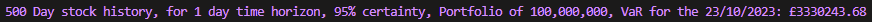
\includegraphics[width=1\textwidth]{Images/Historical Command Line Result.png}
    \caption{Historical Simulation VaR Result}
    \label{fig:Historical Command Line Result}
  \end{figure}

For this project, I did not look up any online VaR results for this stock or any other further stock used, since I believe the methods were robust enough to be reliable. Since I also create multiple methods for calculating VaR, I was able to cross-reference them with each other, with them mostly showing similar results for the same stock, so I am confident that 
these are accurate VaR predictions.

\subsubsection{Command Line -- Model Building  (Variance-Covariance)}

To begin with this method, I discovered that I could import the historical stock price data conveniently by using the \href{https://pypi.org/project/yfinance/}{yfinance} package, which provides a convenient way to download financial market data from Yahoo Finance directly into Python. I selected Nike (NKE) as the target stock so I could compare it to the previous result given by Historical Simulation. A time span of the last 500 trading days was once again chosen to balance between a sufficient data sample size and computational efficiency, as well as for comparative reasons.\\\vspace{0.3cm}

The first step was to import the necessary libraries and download the stock data using the \texttt{yf.download()} function, one of these additional libraries being scipy, which is a used for scientific and technical computing, due to it allowing the user to manipulate and visualize data with a wide range of high-level commands, one of such being the \texttt{norm.ppf()} function, which is used to calculate the inverse of the cumulative distribution function (CDF) of the normal distribution, also known as the Percent Point Function (PPF) that I will need to utilise in a future step. I then discovered that you can use the inbuilt \texttt{pct\_change()} function to calculate the daily returns/percentage changes for the whole data set, which is a much more efficient way of doing it than the method I used for Historical Simulation. I also used the \texttt{dropna()} function to remove any missing values from the data set, in case using the API rather then the CSV could cause this issue.\\\vspace{0.3cm}

\begin{verbatim}
  from scipy.stats import norm
  import yfinance as yf
  
  stock = yf.download('NKE', dt.datetime(2021, 10, 26), dt.datetime(2023, 10, 24))
  closeDiffs = stock['Adj Close'].pct_change()
\end{verbatim}

I then proceeded to define the necessary variables to calculate the VaR, following the formula outlined in Equation~\ref{eq:Variance-Covariance VaR}. The portfolio and risk level were set to 100,000,000 and 0.05 (5\%) respectively, since these were the value's used in Historical Simulation, then the mean was calculated using the \texttt{np.mean} function, followed by the standard deviation using the \texttt{np.std} function.\\\vspace{0.3cm}

\begin{verbatim}
  portfolio = 100000000
  rlPercent = 0.05
  mean = np.mean(closeDiffs)
  sD = np.std(closeDiffs)
\end{verbatim}

Finally, calculating the VaR result takes place with the negative portfolio value multiplied by the \texttt{norm.ppf()} function, which takes the risk level, mean, and standard deviation of returns as inputs and outputs a Z-score, which corresponds to the point on the normal distribution curve where the cumulative probability is equal to the risk level, giving us the VaR estimation.\\\vspace{0.3cm}

\begin{verbatim}
  print("500 Day stock history, for 1 day time horizon, 95% certainty, 
         Portfolio of 100,000,000, VaR for the 23/10/2023: £" + 
         str(round(-portfolio*(norm.ppf(rlPercent, mean, sD)), 3)))
\end{verbatim}

The output of this computation provides a VaR estimate under the assumption of normally distributed returns and a linear correlation between the assets. This assumption is a of course a simplification and might not hold during periods of financial turmoil, which I acknowledge as a limitation of the model, but for this data it is acceptably accurate.\\\vspace{0.3cm}

\begin{figure}[h]
  \centering
  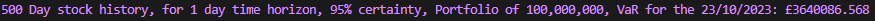
\includegraphics[width=1\textwidth]{Images/Variance-Covariance Command Line Result.png}
  \caption{Variance-Covariance VaR Result}
  \label{fig:Variance-Covariance Command Line Result}
\end{figure}

As you can see, the VaR result is very similar to the one calculated using Historical Simulation, which is a good sign that both methods are accurate. But how do I check the validity of both methods/models?

\subsection{Back-Testing}
So for the methods that I had already coded, I had achieved VaR estimations, but I had no way of validating how accurate they were, which is where back-testing comes in. Back-testing is a way of testing the accuracy of a model by using historical data to see how well it would have predicted the actual results. For example, if I had a model that predicted the weather, I could use back-testing to see how accurate it was by using historical weather data to see how well it has predicted the weather correctly in the past\\\vspace{0.3cm}

To achieve this, you need to see how many times you model has previously predicted the correct VaR, or more so, how many times they have predicted the VaR wrong. To do this, lets say you have 500 days of historical data, and you want to see how many times your model has predicted the VaR wrong for a 1 day time horizon, 95\% certainty, and a portfolio of 100,000,000. 
You would first need to take a portion of the data, lets say the first 50 days, and calculate the VaR for it using the model. You would then compare this VaR result to the actual value that the portfolio lost/gained from the 50th day to the 51st day, thus seeing if the model predicted the VaR correctly. This would then continue, keeping the 50 day data span, but moving it along by 1 day each time, so the next data span would be from the 2nd day to the 51st day, then the 3rd day to the 52nd day, and so on, until you reach the end of the data set. This can be seen in Figure~\ref{fig:Back-Testing} below.\\\vspace{0.3cm}

\begin{figure}[h]
  \centering
  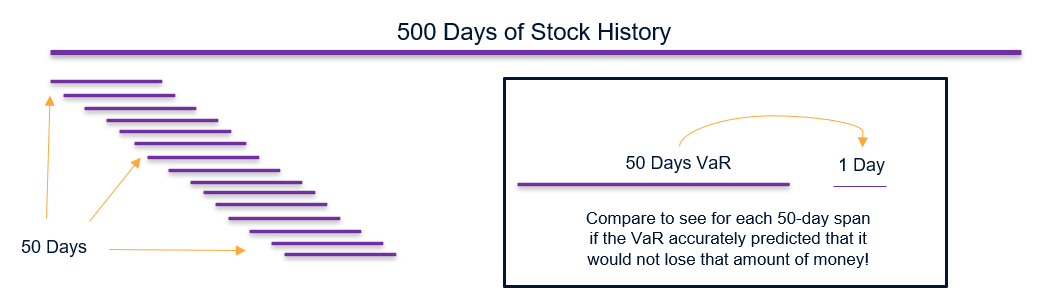
\includegraphics[width=1\textwidth]{Images/Back-Testing.png}
  \caption{Back-Testing Diagram (Source: My Presentation Powerpoint)}
  \label{fig:Back-Testing}
\end{figure}

Every time one of these spans creates a VaR that fails to accurately predict the next days loss, you would make note of it and add it to a counting total. This total can then be utilised with p-values. A p-value is a statistical measure that helps to determine the significance of the results obtained from a hypothesis test. In the context of back-testing, the null hypothesis typically states that the model's predictions are correct, and the alternative hypothesis suggests that the model's predictions are not accurate. A low p-value indicates that the observed data is unlikely under the null hypothesis, leading to its rejection in favour of the alternative hypothesis. So for our VaR back-testing, a low p-value would suggest that the model's performance is not as good as predicted, potentially failing to capture the risk adequately.

To do this within Python whilst leading on from our previous two coded methods, I added the following codee to the end on both models. It creates a variable called \texttt{count}, which is used to count the number of times the model has predicted the VaR incorrectly, and a variable called \texttt{adjust}, which is used to adjust the data span to be used for the VaR calculation, this being 10\% of the data set. It then creates a \texttt{for} loop, which iterates through each day of the data set, calculating the VaR for the data span, then comparing it to the actual value that the portfolio lost/gained from the last day of the data span to the next day, thus seeing if the model predicted the VaR correctly. This will repeat for the length of the entire historical data history, minus the span adjust and minus 1 as well, since you would need to compare 449--499 day VaR to day 449--500's return. The next day return is also multiplied by -1, so it accounts so that the losses are positive like the VaR estimations, making it easy to compare if one is incorrectly larger then the other. If the VaR was predicted incorrectly, the \texttt{count} variable is increased by 1.\\\vspace{0.3cm}

\begin{verbatim}
  count = 0
  adjust = int(len(stock)/10)
  for i in range(1, len(stock) - adjust - 1):
      backTest = stock['Adj Close'].pct_change()[i:i+adjust]
      if Historical Simulation:
          VaR = np.percentile(backTest, rlPercent)*portfolio*-1
      else: #Model Building
          VaR = -portfolio*(norm.ppf(rlPercent, mean, sD))
      nextDay = stock['Adj Close'].pct_change()[i+adjust:i+adjust+1].values[0]
      nextDay = nextDay*portfolio*-1 #Done to fit within Latex Hbox
      if nextDay > VaR:
          count += 1
\end{verbatim}

 Next, I compute the p-value using the cumulative distribution function (CDF) of the binomial distribution, which in turn calculates the probability of observing a certain number of VaR exceedances (or fewer) given the expected number of exceedances under the model's assumptions.\vspace{0.3cm}
 
 \begin{verbatim}
  pValue = binom.cdf((len(stock)-adjust)-count,len(stock)-adjust,1-rlPercent/100)
  \end{verbatim}

 The parameters for the \texttt{binom.cdf} function are as follows:

\begin{itemize}
    \item The number of successes, which is the total number of days minus the adjustment for the data window and the count of exceedances.
    \item The number of trials, which is the length of the stock data minus the adjustment for the data window.
    \item The probability of success on each trial, which is 1 minus the risk level percentage divided by 100, reflecting the confidence level of the VaR estimate.
\end{itemize}

The calculated p-value is then compared to the risk level percentage to determine the statistical significance. If the p-value is greater than the risk level percentage, the model passes the back-test, indicating that the number of VaR exceedances is within acceptable limits of the model's predictions. Conversely, a p-value lower than the risk level percentage suggests that the model's poor predictive performance is statistical significance, and it fails the back-test.[\ref{ref11}]

\begin{verbatim}
if pValue > rlPercent/100:
    print("Back Test: PASSED with " + str(round(pValue*100, 0)) + 
    "% statistical significance level (p-value)")
else:
    print("Back Test: FAILED with " + str(round(pValue*100, 0)) + 
    "% statistical significance level (p-value)")
\end{verbatim}

By utilizing p-values, we can assign a level of confidence to our back-testing results, supporting the validation process of our VaR model. It enables us to make informed decisions about the model's reliability and whether it can be trusted for making future risk assessments. It help provide a quantitative method to validate the accuracy of VaR models, ensuring that risk managers and financial analysts can rely on the model's predictions to make critical decisions. In the future, along a set of portfolio's with multiple stocks within, I could perform multiple back test on multiple stocks using both VaR, and form a statistical conclusion on how many time each model fails the p-value back-testing, thus seeing which model is more reliable and should possibly be used in further graphical builds, although I have not touched on Monet Carlo simulation yet, which could be far more accurate then either of these two methods, so I will have to see how my research into it goes.[\ref{ref11}]

\begin{figure}
  \centering
  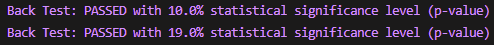
\includegraphics[width=0.7\textwidth]{Images/Back-Testing Results.png}
  \caption{Results using Tesco stock data, for Historical Simulation followed by Model Building.}
  \label{fig:Back-Testing Results}
\end{figure}

\subsection{Combining Implementations}
Before I decided to embark on the creation of any of my graphical elements, I thought it would be good to have some way to test my VaR models on different single stocks, so I could see a range of results, and better gauge the consistency levels of my back-tests, as well as also being able to simple see more VaR results then just what I had seen so far. I created a fully functioning command line program that allows the user to select a stock from the FTSE100 list (I chose this as I do not have a wide knowledge of stock lists, but since I knew of this one already and all the stocks on it are significant, it would be good to implement), enter a given portfolio value that they would have invested within this one particular stock, and then select a time horizon and confidence level for the VaR calculation. It would then give them 3 options for how much historical data they would want to use, either 100, 500 or they could input their own dates, and it would finally ask what model they would like to compute the VaR estimation with, either Historical Simulation or Model Building. It would compute the VaR and then display the result, as well as display the p-value back-testing result.\\\vspace{0.3cm}

Since the code for this is just a large and robust amount of verification and input statements, I will not include it in this report, but I will display a full interaction in figure~\ref{fig:Single Stock VaR}. I used pandas to retrieve the FTSE100 from Wikipedia, pandas being a powerful data manipulation library in Python, allowing for web scraping, reading and writing data, which I utilised it for in this case. Everything else included within the code has been covered within previous pages within this chapter. Full interaction found on the next page:

\begin{figure}
  \begin{verbatim}
    WELCOME TO THE VAR CALCULATOR
    -----------------------------
    Which companies stock would you like to calculate the VaR for?
    1 - 3i
    2 - Admiral Group
    3 - Airtel Africa
    ...
    40 - Haleon
    41 - Halma plc
    42 - Hargreaves Lansdown
    43 - Hikma Pharmaceuticals
    44 - Howdens Joinery
    ...
    97 - Vodafone Group
    98 - Weir Group
    99 - Whitbread
    100 - WPP plc
    Enter the number of the company: 42
    Enter the portfolio value (£): 100000000
    Enter the risk level percentage (1%, 5%, etc.): 5
    Enter the time horizon (Max: 100 days): 1
    How many days of historical data would you like to use, 
    or would you like to choose your own date boundaries?
    1. 100 days
    2. 500 days
    3. Choose your own
    Enter the number of your choice: 2
    [*********************100%%**********************]  1 of 1 completed
    Would you like to calculate VaR using Historical Simulation, 
    or using Model Building/Variance-Covariance (H/M): m
    
    VaR is: £5,818,845.68
    Back Test: PASSED with 32.0% statistical significance level (p-value)
  \end{verbatim}
  \caption{Console output of the Single Stock VaR.py program.}\label{fig:Single Stock VaR}
\end{figure}

 I have neglected to mention how the Time Horizon in handled within this program. The best way to show how it is handled would be to quote from reference [\ref{ref6}] --- \textit{Options, Futures, and Other Derivatives.} by John C. Hull, which states:

 \begin{quote}
  VaR has two parameters: the time horizon \( N \), measured in days, and the confidence level \( X \). In practice, analysts almost invariably set \( N = 1 \) in the first instance. This is because there is not enough data to estimate directly the behavior of market variables over periods of time longer than 1 day. The usual assumption is: 
  \begin{equation}
    N\text{-day VaR} = \text{1-day VaR} \times \sqrt{N}
    \label{eq:Time Horizon}
  \end{equation}
  This formula is exactly true when the changes in the value of the portfolio on successive days have independent identical normal distributions with mean zero. In other cases, it is an approximation.
\end{quote}
  
  Since VaR is scaled with time due to volatility. Volatility tends to be proportional to the square root of time.
  \begin{equation}
    \text{Volatility(Time)} = \text{Volatility(One Period)} \times \sqrt{\text{Time Horizon}}
    \label{eq:Volatility}
  \end{equation} 

  Since we are dealing with the other cases frequently throughout the use of the VaR Models used within the programs, I utilise the formula \ref{eq:Time Horizon} above to accommodate for the VaR value over a given time period, by multiplying the VaR by the square root of the given time horizon, which is why the user is asked to input the time horizon in days, and not in years or months, this providing sufficient estimations so far.

% \subsubsection{Multiple Stocks}
\newpage
\section{Chapter 3 --- Graphical User Interface}

\subsection{What is Kivy?}
Kivy \href[page=1]{https://kivy.org/#home}{(https://kivy.org/)}is an open-source Python library for developing multitouch application software with a natural user interface (NUI). It is highly versatile and can run on various operating systems, including Windows, macOS, Linux, Android, and iOS\@. This cross-platform compatibility is due to Kivy's use of OpenGL ES 2, allowing it to render consistent graphics across all supported platforms.[\ref{ref9}] Kivy is also free to use, even for commercial purposes, as it is distributed under the MIT license.\\\vspace{0.3cm}

Kivy's compatibility with multiple operating systems makes it an excellent choice for financial software development. The ability to write code once and deploy it on various platforms without modification is particularly advantageous in a financial context, where users may access software from different devices.

\begin{itemize}
    \item \textbf{Cross-Platform:} Kivy apps can run on desktop and mobile devices, enhancing accessibility for users who need to monitor financial markets or run VaR calculations on the go.
    \item \textbf{Pythonic Nature:} Given that Python is a leading language in financial modelling due to its simplicity and the powerful data analysis libraries available, Kivy integrates well within the Python ecosystem, as well as it being the chosen language for this project.
    \item \textbf{Graphics Engine:} Kivy's graphics engine is built over OpenGL ES 2, providing the capability to handle intensive graphical representations, which is essential for visualizing complex financial data that I will want to do in the future.
\end{itemize}

Developing financial software with Kivy brings several benefits:

\begin{itemize}
    \item \textbf{Rapid Development:} Kivy's straightforward syntax and powerful widgets allow for rapid development of prototypes and software, which is crucial in the fast-paced environment of financial markets.
    
    \item \textbf{Multitouch Support:} The library's inherent support for multitouch can be leveraged to create interactive financial dashboards, enhancing data exploration and manipulation for important tasks such as risk analysis which we will want to use it for.[\ref{ref9}] 
    
    \item \textbf{Customizable UI:} Kivy provides the tools to create a highly customizable user interface (UI), enabling the development of aesthetic financial applications tailored to the specific needs of financial analysts.
    
    \item \textbf{Community and Support:} Kivy has a growing community and good documentation, which will be highly useful for me as a beginner to the library.
\end{itemize}

Kivy presents itself as a robust framework for financial software development. Its compatibility with different operating systems, ease of operation within Python, and the capability to create sophisticated UIs make it an appealing choice for developers such as myself to use when creating financial applications, especially when catered for VaR analysis and other risk management tools, which is why I've chosen to use it for this project for the GUI.\@

\subsection{Conceptualisation of Initial Design Ideas}

The initial design phase of the Value at Risk (VaR) calculation tool will focus on creating a tool that will allow the user to interact with it in an efficient and effective manor, with less of an emphasis on a visually pleasing design, more on practicality for what has been researched and commented on so far. I had an idea in mind for what I wanted to initially be able to create, so I decided to create a design sketch (Figure~\ref{fig:InitialDesignSketch}), which reflects an early conceptualization of the interface, emphasizing simplicity and functionality.

\begin{figure}[h]
  \centering
  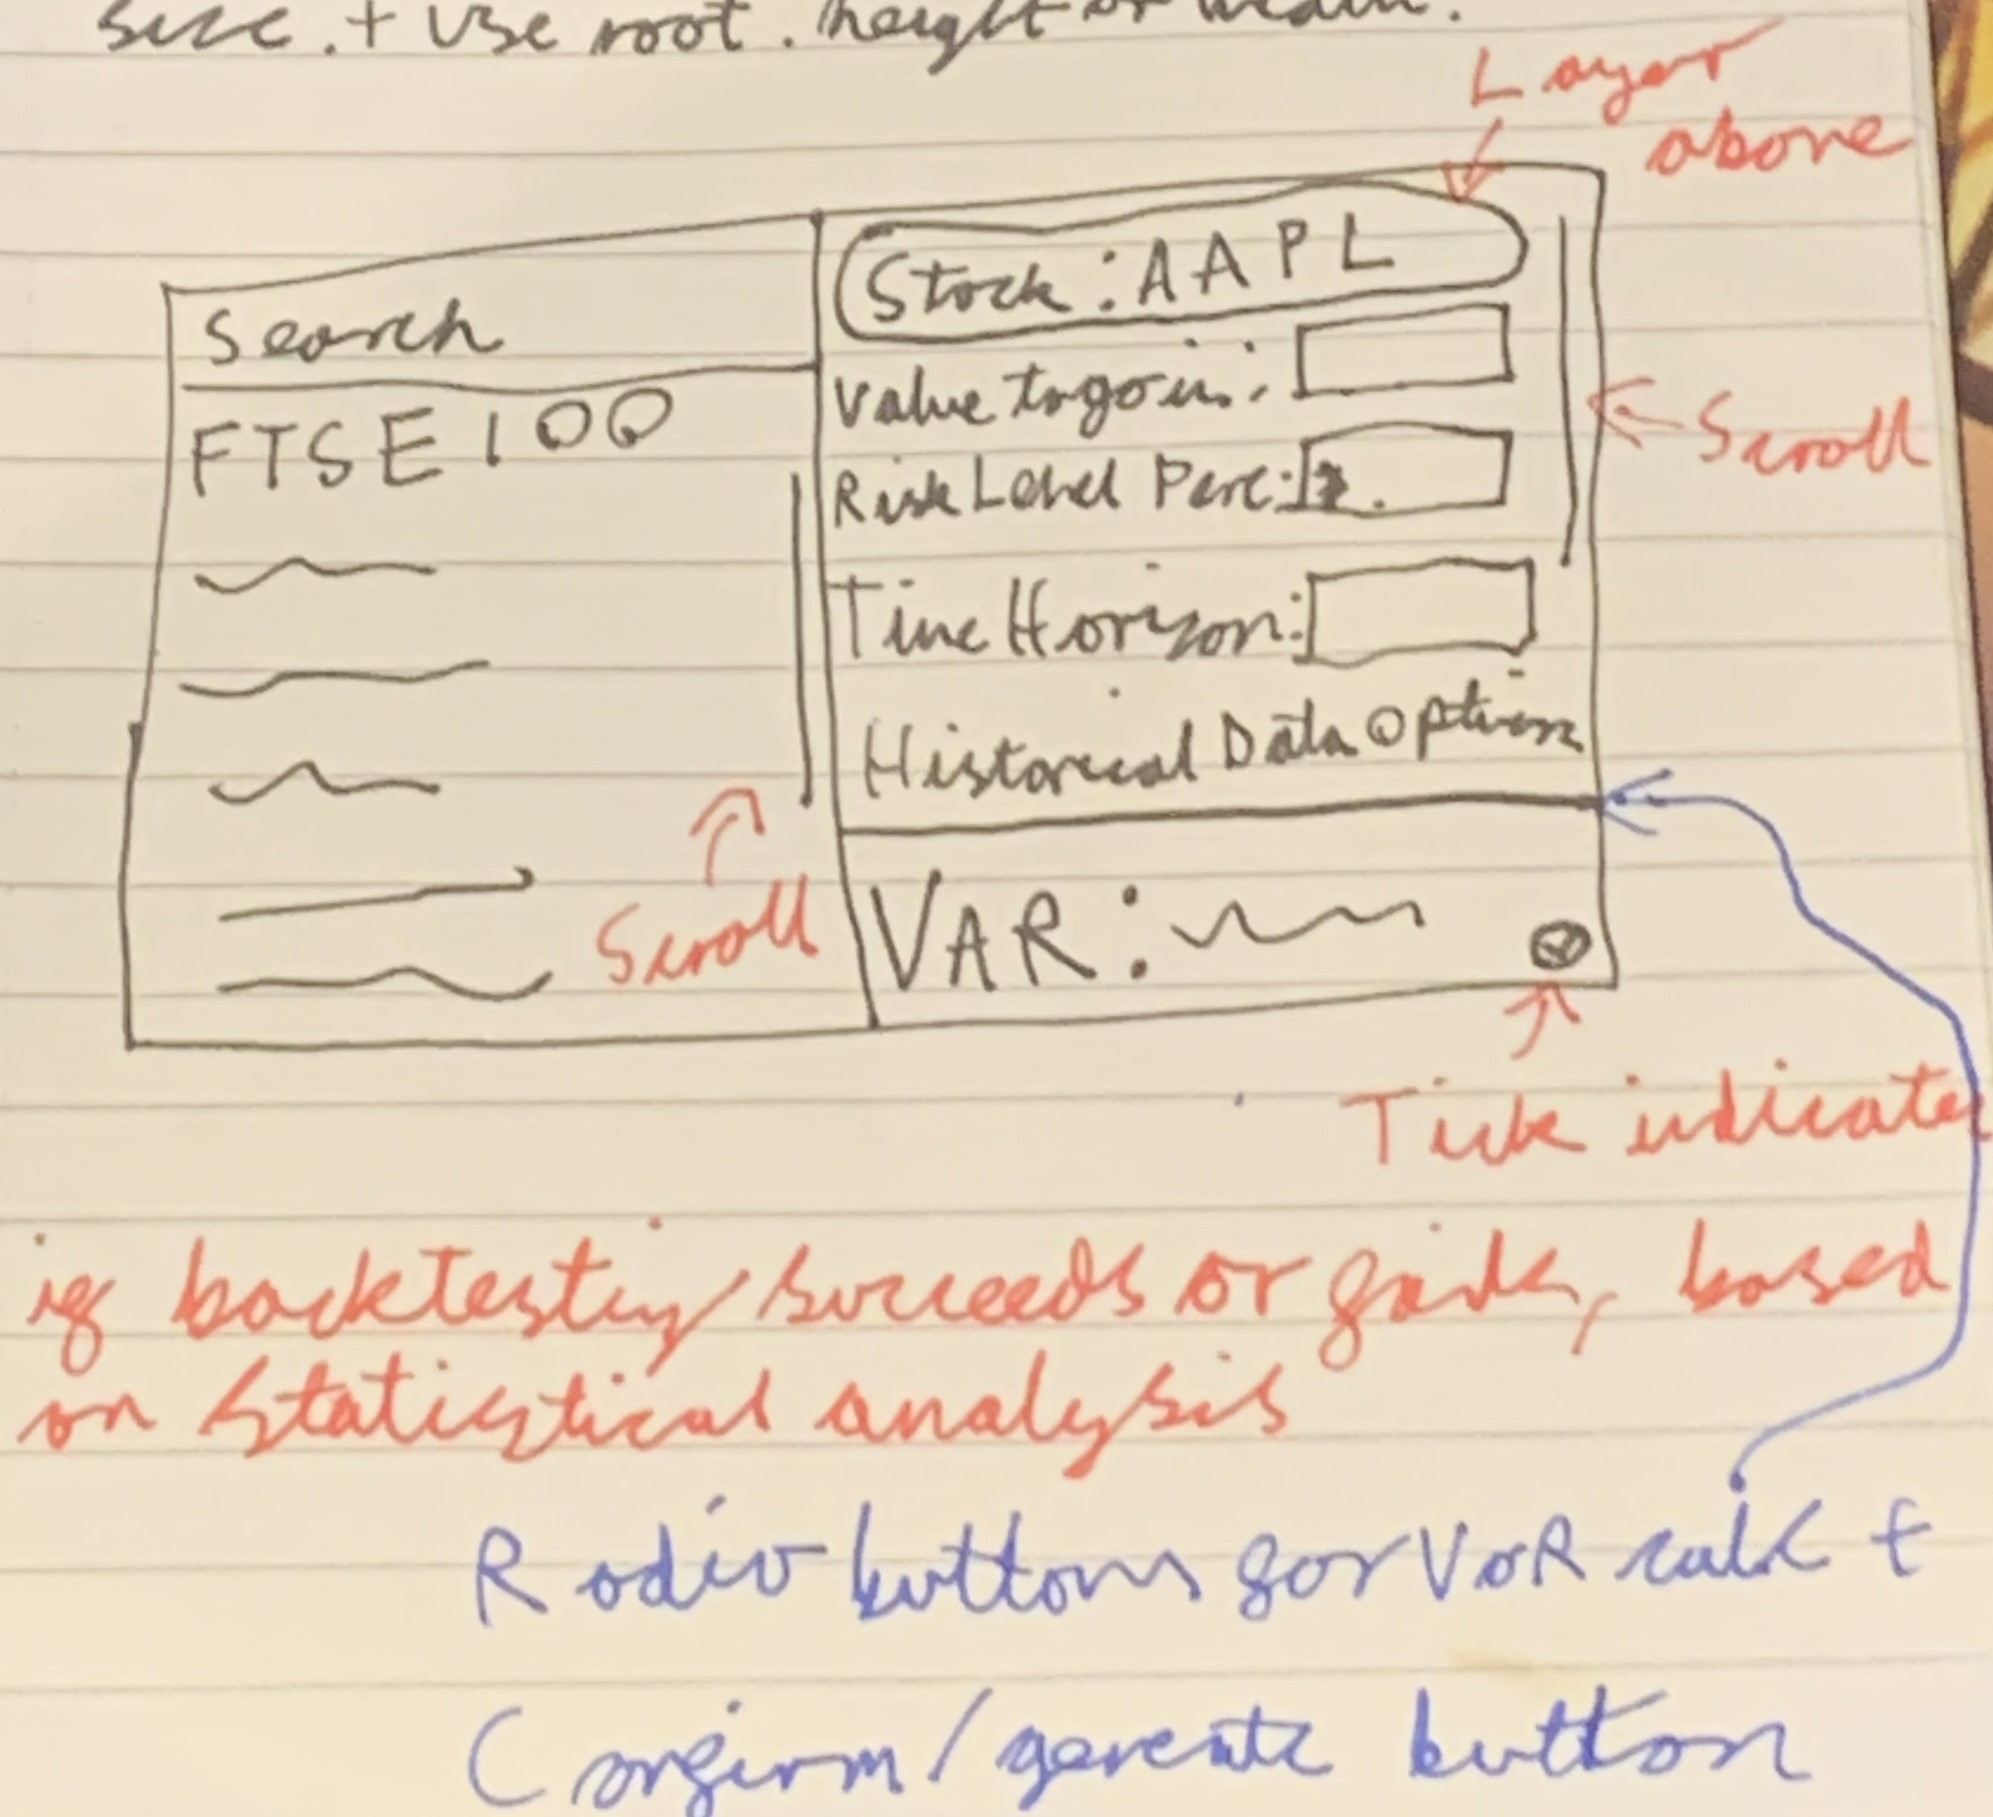
\includegraphics[width=0.7\textwidth]{Images/Initial Design Sketch.jpg}
  \caption{Initial GUI Design Sketch}
  \label{fig:InitialDesignSketch}
\end{figure}

The layout was envisioned to comprise of two main sections: a search and selection panel on the left and an input/detail panel on the right. The search panel allows users to filter and select stocks from the FTSE100 to then be used on the right, as well as search for any stock that they want from an autocomplete database. The detail panel on the right is structured to enable users to specify parameters for the selected stock, such as portfolio value, risk level percentile, time horizon and what VaR model you want to use. A scroll feature could also be implemented to accommodate future desired adjustable parameters, such as historical data options. Below the scroll is a fixed section that will display the final VaR after the rest of the informational parameters have been interacted with/data has been submitted into them. There will also be a tick to indicate if back-testing's hypothesis through statistical analysis had been rejected, this influencing if this model with this stock passes.\\\vspace{0.3cm}

A key feature highlighted in the sketch is the inclusion of the layered "current stock" display in the top right, as it lets the users easily see what they have selected, whilst also letting the scroll move underneath it, helping the program look and act dynamically. Additionally, a tick indicator was conceptualized to provide immediate visual feedback when back-testing succeeds or fails, based on statistical analysis (p-values), enhancing the user's understanding of the model's performance, showing evidence of system status. The design also incorporates radio buttons for VaR calculation modes for historical and model-based approaches, allowing for quick toggling between different methods whilst still maintaining the other pre-selected parameters.\\\vspace{0.3cm}

This initial design was guided by principles of user centered design (UCD) best practices, aiming to streamline the complex process of risk analysis into a manageable and approachable workflow for end-users. Each element was chosen for its potential to make the software accessible to both novice and experienced users, allowing for ease of user regardless of skill level.\\\vspace{0.3cm}

The conceptualisation phase was pivotal in laying the groundwork for the subsequent development of this GUI. It helped me visualise how it needed to look and how the interactions would have to take place, so even if the final result wasn't visually the same, it still provided an excellent user story for how it needed to perform.

\subsection{Initial GUI Creation}
Before my initial creation, I followed a lot of the book [\ref{ref9}], \textit{Kivy - Interactive Applications and Games in Python - Second Edition} by Roberto Ulloa, which I have referenced in my bibliography, as it was a very useful book for learning the basics of Kivy, and I would highly recommend it to anyone who wants to learn Kivy.

\subsubsection{First Iteration}
Since the book taught me to seperate the GUI into two files, I have done so for my baseline of the application, these files  being the .py file, which contains the code for the GUI, and the other being the .kv file, which contains the layout and styling of the GUI, I will be explaining the code for both of these files, as well as the code for the main.py file, which is the file that runs the GUI.\@\\\vspace{0.3cm}

The Python script `Initial Design Test.py' serves as the backbone of the application. Utilizing Kivy's standard libraries, the script defines my ApplicationView class, which inherits from Kivy's BoxLayout to establish the fundamental structure of the GUI:

\begin{verbatim}
class ApplicationView(BoxLayout):
    stockList = ObjectProperty(None)
    userInputs = ObjectProperty(None)
    ...
    def populateList(self):
        ...
    def populateInputs(self):
        ...
\end{verbatim}

The `ApplicationView' class is integral to the GUI, as it initializes the user interface and binds the graphical components to the backend logic. The ObjectProperty instances `stockList' and `userInputs' are object placeholders for dynamic python elements within the GUI.\@ The methods `populateList' and `populateInputs' are responsible for filling these placeholders with actual content — in this case, labels representing stock data and text input fields for user parameters, respectively.\\\vspace{0.3cm}

The layout and styling of the GUI are defined in the Kivy language file `IDT.kv', which allows for a clear separation of the interface design from the logic of the application:

\begin{verbatim}
<ApplicationView>:
    orientation: 'horizontal'
    BoxLayout:
        orientation: 'vertical'
        ...
        ScrollView:
            ...
\end{verbatim}

This .kv file outlines two main sections in a horizontal arrangement — a searchable stock list and a detailed input area for configuring VaR parameters. The use of ScrollView elements ensures that the content is accessible even when it exceeds the screen space. This design decision was made to enhance the application's scalability and to provide a seamless user experience.\\\vspace{0.3cm}

The `populateList' and `populateInputs' functions demonstrate the dynamic nature of the interface. They are called upon initialization to populate the GUI with interactive elements:

\begin{verbatim}
def populateList(self):
    for i in range(100):
        self.stockList.add_widget(Label(...))
        
def populateInputs(self):
    for i in range(20):
        self.userInputs.add_widget(Label(...))
        self.userInputs.add_widget(TextInput(...))
\end{verbatim}

These functions are responsible for creating the labels and text input fields that are displayed in the GUI.\@ The labels are populated will hopefully be populated stock data, and the text input fields will be used to configure VaR parameters.  This approach allows for the creation of a scalable interface that can be easily adapted to accommodate additional stocks and parameters in the future, once they are implemented.\\\vspace{0.3cm}

Upon executing the `Initial Design Test.py' script, the Kivy application builds the GUI based on the defined classes and .kv file, initiated by the following code:

\begin{verbatim}
if __name__ == '__main__':
    IDTApp().run()
\end{verbatim}

\begin{figure}[h!]
  \centering
  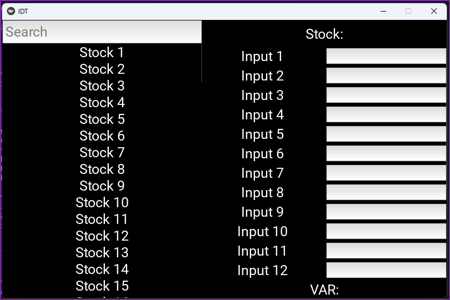
\includegraphics[width=0.8\textwidth]{Images/Initial Design Test Image 1.png}
  \caption{Initial Design Test - First Iteration}
  \label{fig:Initial Design Test - First Iteration}
\end{figure}

\newpage
\subsubsection{Final Iteration}
For my final iteration of the design, I took all of the elements that were explored within the Combining Implementations chapter, and implemented them into the GUI, as well as adapting some of the old features so they could work in the boundary of what I was able to achieve. I would explain some of the code for both of the .py and .kv files respectively.\@\\\vspace{0.3cm}

However, I do not feel that I have adequate time left when writing this to explain all of the code for both the files, like I have in previous sections. I plan to cover the code in full detail in my final report. Instead, I will show images of this final iteration of the initial design, explaining my thoughts on the compromises I had to make (such as removing the search feature in the top left and the scrolling ability of the right hand side), and what I would like to improve on in the future. I will also include a link to a Youtube video that showcases various interactions with the programs. Finally, I plan to briefly touch on a few elements from the code when I discuss some of the Design Patterns that I implemented within it.\\\vspace{0.3cm}

I used pyInstaller \href[page=1]{https://www.pyinstaller.org/}{(https://www.pyinstaller.org/)} to create an executable file for the GUI, which can be found within the base folder for this project, which can be run on any Windows computer. I will work on having the visual accessibility to be able to port my future GUI's onto mobile devices. The .exe also opens up a console whilst the program runs, I cannot seem to get the program to work without crashing when I disable the console, so I will try and fix that for next term. As another final thing to add, I have left heavy comments within the code helping to explain certain sections, as is such with good software engineering practices.\\\vspace{0.3cm}

\begin{figure}[h!]
  \centering
  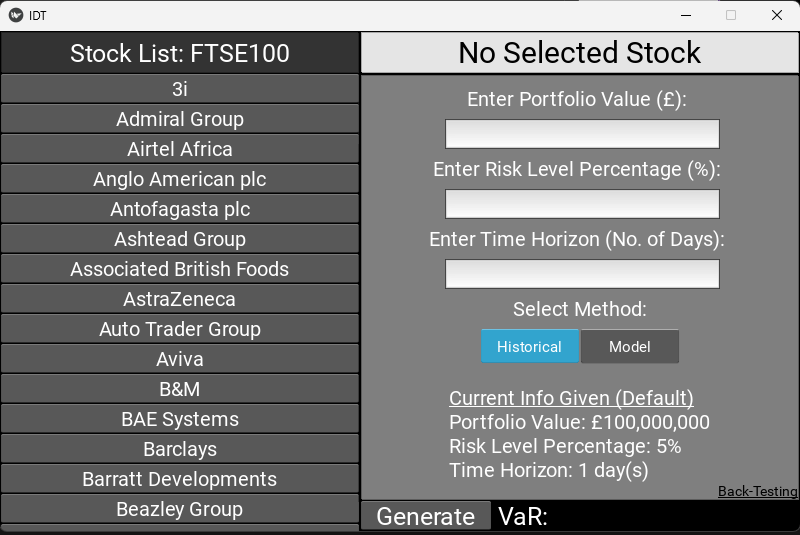
\includegraphics[width=0.8\textwidth]{Images/Initial Design Tes - Final Iteration 1.png}
  \caption{Initial Design Test - Final Iteration 1}
  \label{fig:Initial Design Test - Final Iteration 1}
\end{figure}

\begin{figure}[h!]
  \centering
  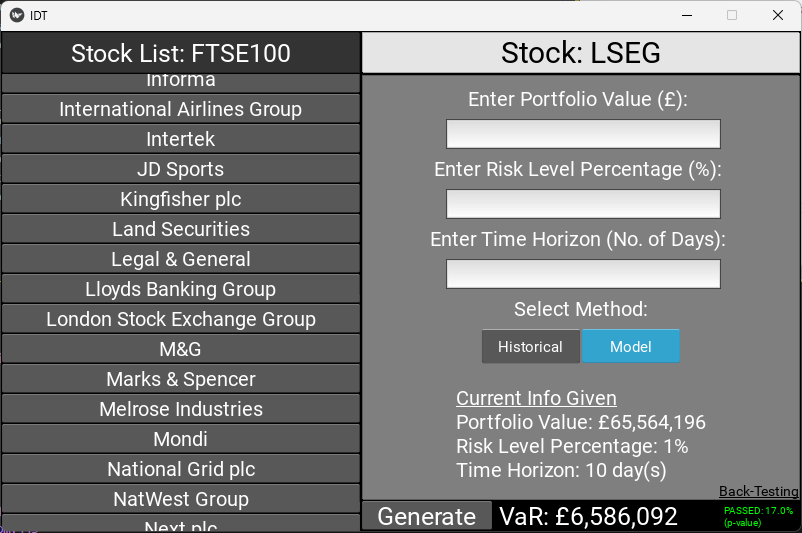
\includegraphics[width=0.8\textwidth]{Images/Initial Design Tes - Final Iteration 2.png}
  \caption{Initial Design Test - Final Iteration 2}
  \label{fig:Initial Design Test - Final Iteration 2}
\end{figure}

Youtube Video: \href{https://youtu.be/2GIWug_IESI}{Presentation Demonstration For FYP}

% \subsection{GUI Practicality \& Industry Comparisons}
% Explain the uses of the GUI, and delve into the fact you need to look up what other ones do for next turn

% \subsection{Testing and Refinement}


\section{Chapter 4 --- Software Engineering}

\subsection{Design Patterns}

In developing my Initial Design for my Graphical User Interface (GUI) to calculate VaR, I have employed several design patterns that facilitate a robust, scalable, and maintainable codebase. Below are key design patterns utilized within my application:\\\vspace{0.3cm}

\underline{\textbf{Model-View-Controller (MVC)}}\\\vspace{0.3cm}

For my final iteration of my Initial GUI Design, the architecture loosely follows the MVC pattern, segregating the application logic (Model), user interface (View), and input control (Controller) into separate components. This separation enhances the application's ability to handle user interactions and data manipulation independently.

\begin{itemize}
    \item The \textbf{Model} is represented by the data retrieval and VaR calculation logic, which fetches financial data and computes the VaR and back-testing estimation.
    \item The \textbf{View} is the user interface, designed with Kivy's layout and widget system, providing a responsive and interactive experience.
    \item The \textbf{Controller} is evident in the event-handling methods, like \texttt{populateList} and \texttt{generateVaR}, which respond to user inputs and trigger model updates.
\end{itemize}

\underline{\textbf{Observer Pattern}}\\\vspace{0.3cm}

The Observer pattern is present in the way the application monitors the state of user inputs. For instance, toggle buttons for selecting the VaR calculation method employ event listeners that update the system's state when user interaction occurs.

\begin{verbatim}
hButton.bind(on_press=self.simMethodPressed)
mButton.bind(on_press=self.simMethodPressed)
\end{verbatim}

This pattern decouples the system's components, allowing for independent updates and scalability.\\\vspace{0.3cm}

\underline{\textbf{Command Pattern}}\\\vspace{0.3cm}

The Command pattern is utilized in encapsulating the action to be performed in response to user interactions. For example, when a user selects a stock or initiates a VaR calculation, the corresponding actions are enclosed within command methods, such as \texttt{populateList} or \texttt{generateVaR}.

\begin{verbatim}
button.bind(on_release=lambda btn, i=i: ...)
\end{verbatim}

This approach allows for more flexible and extensible execution of actions within the application.\\\vspace{0.3cm}

\underline{\textbf{Singleton Pattern}}\\\vspace{0.3cm}

While not explicitly implemented, the Singleton pattern is conceptually used in the management of the application state. There is only one instance of the \texttt{ApplicationView} class, which maintains a single state throughout the application's lifecycle.

\begin{verbatim}
class IDTApp(App):
    def build(self):
        return ApplicationView()
\end{verbatim}

This ensures that there is a consistent state that is accessible throughout all parts of the application.\\\vspace{0.3cm}

These design patterns contribute significantly to the application's robustness, allowing for efficient risk assessment and providing a foundation for future enhancements and scalability.By adhering to these established practices, I have ensured that my software remains maintainable and adaptable to the evolving needs that my graphical interface my undergo in the future.

\subsection{Testing}

Testing is a critical component of software development, essential for ensuring that the application meets its requirements and is free of errors. Mainly for my project, the primary mode of testing involved running the application and observing its behavior for errors or incorrect VaR calculations.\\\vspace{0.3cm}

This testing approach used can be classified as Ad Hoc Testing and Exploratory Testing. These methods are informal and unstructured, as I have been relying on my intuition and experience to identify issues.

\begin{itemize}
    \item \textbf{Ad Hoc Testing}: This type of testing is carried out without any formal test plan or test case documentation. It is a random examination of the application, often useful for discovering glaring issues quickly.
    \item \textbf{Exploratory Testing}: This approach combines learning, test design, and test execution into a single activity. It is particularly effective in situations where there are no detailed specifications, and tests need to be devised on the fly.
\end{itemize}

While these methods can be effective for identifying obvious faults, they lack reliability and cannot provide a systematic approach that other testing methods would. They are often more suited to the early stages of development which this project is still in, thus me using them so far.\\\vspace{0.3cm}


One of the main limitations of my current testing approach is the absence of \textbf{Test-Driven Development (TDD)}. TDD is a modern software development process where requirements are turned into very specific test cases, then the software is improved to pass the new tests. This approach was not followed, as I was unable to justify what I would be testing for (I had planned out unit testing, but I especially did not know how to incorporate it within a Kivy application, as I have not done TDD with Python or Kivy before), so I continued with the above testing style, which worked and allowed me to create my program efficiently, but not up to the industry standard that I know I should be aiming for.\\\vspace{0.3cm}

\newpage
For future development cycles, I plan on incorporating more testing strategies to enhance the quality and reliability of the application, such as:

\begin{itemize}
    \item \textbf{Unit Testing}: Develop tests for individual components or functions to ensure they work correctly in isolation. (Had already planned, now I shall be able to implement)
    \item \textbf{Integration Testing}: Test the interactions between different parts of the application to verify that they work together as intended (Happened during my Ad Hoc Testing often, but need to be able to explicitly show that that's what I was testing for).
    \item \textbf{Automated Regression Testing}: Implement an automated test suite that can be run regularly to catch regressions early in my next GUI's development cycle.
    \item \textbf{Performance Testing}: Evaluate the application's performance, especially when handling large datasets or performing complex calculations, to ensure that it meets the necessary speed and efficiency requirements, especially when I incorporate multiple stocks, portfolios, and full searching capabilities into future applications.
    \item \textbf{User Acceptance Testing (UAT)}: Involve end-users to validate the functionality and usability of the application in real-world scenarios (Will bring in external individuals to help be observed, providing a wide range of feedback that I can take note of and apply to my application).
\end{itemize}

By integrating these practices, my project can achieve a higher level of quality assurance and deliver a more robust and user-trusted VaR product.

\subsection{Version Control (Git)} 

Version control is a system that records changes to a file or set of files over time so that specific versions can be recalled later. In this project, I have had Git employed as the version control system for everything I have done.
Git is a distributed version control system, which means that the complete codebase and history are available on every developer's computer, allowing for easy branching and merging. My approach to using Git was straightforward:

\begin{itemize}
    \item Regular Commits: Consistent commits were made to the repository, with detailed messages that clearly described the changes and their impact on the project.
    \item Backup and Security: All the code was backed up on OneDrive as well (a personal decision), providing an additional layer of security and ensuring that no work would be lost in case of system failures.
    \item Branching Strategy: While currently the project has not utilised extensive branching, I acknowledging the  benefits of feature branches and plan to rigorously employ them in the future.
\end{itemize}

The practice of making regular commits with detailed messages is incredibly invaluable, thus me making sure to regularly comply with this methodology. It enabled the tracking of changes and helps simplify the process of understanding the evolution of the codebase. For me, Git has been essential for several reasons:

\begin{itemize}
    \item \textbf{Reversion}: Git can allow me to revert to previous states of the codebase, which is crucial when a new feature can accidentally break functionality.
    \item \textbf{Traceability}: With Git, all my changes are traceable to a specific commit, making it easier to track when and why changes were made.
    \item \textbf{Backup and Restore}: My files are backed up on a remote repository, providing a fail-safe in case the my local repository suffers a setback.
\end{itemize}

While my development with this project's version control strategy was effective to a degree, it also highlighted areas for improvement. Adopting a more structured approach to branching and leveraging the full suite of features offered by Git will be a focus in future endeavours to ensure a more efficient and error-preventative development workflow.

% \section{Chapter 5 - Evaluation \& Scope}

% \subsection{Current Work}

% \subsection{Future Work}

\section{Self Evaluation}
In the end, for this term, I am still happy with the progress I made. I learnt some very valuable lessons, such as needing to make sure that I do all of the documentation alongside the coding, since with the gap in progress, it can become tedious to try and explain it all properly in the future. I feel that I accomplished the goals set out within my original timeline for what I wanted to achieve this term, for this interim report, and whilst there are sections of this report that I am unhappy with the result of (especially the final iteration of the GUI), I am still satisfied with the report as a whole in displaying what I had learnt and the code I was able to create, especially with the inconsistency with my physical and mental health experienced over the last few months. I also am aware of my lack of testing that I have performed, I spent a large chunk of time just testing everything myself to make sure it works, when I should have been following a better framework, I plan to learn from this and change the way I develop and document the code come next term. I know the Latex is not great in this document, its still the first time I've ever done large scale documentation like this before, but hopefully by the time my final report is complete I will have given myself enough time for it to be at an acceptable level. I also know I haven't used enough sources, the sources that I did use were so useful that I kept referring back to them, which makes my ability to reference them rather bland, so I will also make sure to diversify with many more references in the future. With how the final design for the initial GUI came out, I'm extremely happy with its functionality, its very fast and easy to use and produces the exact results you need whilst still being robust. There's still a lot to work on for it in the future, like adding different windows/views, incorporating multiple stocks VaR calculations (I wrote a program to do multiple stocks but I didn't have the time to include that in this documentation either, can be found within my Git project/submitted programs) and allowing you to access entire portfolio's within the application. What I made this term was a great proof of concept for what I can do with Kivy, for my final report I want to be able to do so much more, since that is my main goal, the development of an industry grade application for Value at Risk as well as financial management in general. Finally, there were many planned sections of this report that were never completed, I aim to be able to structure my documentation so that I can complete everything I need in the following term, so to conclude, I am extremely happy with everything I was able to do, but I plan on doing everything much better in the future, as I know it was not optimal enough for what I want to achieve...

% \subsection{VaR and what it is in the industry atm, and other VaR softwares and how I can take inspo from them?}
\newpage
\section{Bibliography}
\begin{small}
\begin{enumerate}
  \item\label{ref1} Alexander, C. (2008). *Market Risk Analysis: Value-at-Risk Models.* Hoboken, NJ: Wiley. [Online] Available at: \url{https://ebookcentral-proquest-com.ezproxy01.rhul.ac.uk/lib/rhul/reader.action?docID=416450}.
  \\\textit{This book covers various aspects that I want to approach in this project, such as historical simulation, Monte Carlo simulation and various forms of testing that could be highly useful for my project.}
  
  \item\label{ref2} Arbuckle, D. (2017). *Daniel Arbuckle’s Mastering Python: Build Powerful Python Applications.* Birmingham, England: Packt. [Online] Available at: \url{https://learning.oreilly.com/library/view/daniel-arbuckles-mastering/9781787283695/?ar=}.
  \\\textit{I chose this reference as it helps with python packaging, being able to turn a python code and all its GUI and libraries into a single executable file, which is something I want to be able to do for this project.}

  \item\label{ref3} Choudhry, M. (2006). *An Introduction to Value-at-Risk.* Chichester: John Wiley \& Sons Limited. [Online] Available at: \\ \url{https://learning.oreilly.com/library/view/an-introduction-to/9780470017579/}.
  \\\textit{Covers similar topics to the first reference, but seems to go into more detail on specific issues that I may need to address in this project.}
  
  \item\label{ref4} Duffie, D. and Pan, J. (2019). *An Overview of Value at Risk.* [Online] Available at: \url{http://web.mit.edu/people/junpan/ddjp.pdf}.
  \\\textit{A much shorter reference, it is a paper that covers the basics of Value at Risk, which I will be using to help me understand the fundamentals of the topic since I have been able to follow it better then the other references.}
  
  \item\label{ref5} Föllmer, H. and Schied, A. (2016). *Stochastic Finance: An Introduction in Discrete Time.* Berlin: de Gruyter. [PDF]
  \\\textit{A recommended reference from my supervisor, it is a book that covers higher level concepts relating to my project but also provides an overview of stochastic finance in general, which I have seen to be useful in understanding the topic.}
  
  \item\label{ref6} Hull, J.C. (2008). *Options, Futures, and Other Derivatives.* Upper Saddle River, NJ: Prentice Hall. [PDF]
  \\\textit{This is my main reference for the project, as it is the main textbook suggested. It has a relevant chapter on Value at Risk, which explores many of the different aspects that I will need to look into for this project.}

  \item\label{ref7} Pritsker, M. (1997). "Evaluating Value at Risk Methodologies: Accuracy versus Computational Time." *Journal of Financial Services Research* 12: 201-242. [Online] Available at: \url{https://doi.org/10.1023/A:1007978820465}.
  \\\textit{Another short reference, this is a paper that compares the accuracy and computational time of various Value at Risk methodologies, which I will be using to help me understand the different methodologies and how I can apply them to my project in the most efficient manner.}

  \item\label{ref8} Raman, K. (2015). *Mastering Python Data Visualization: Generate Effective Results in a Variety of Visually Appealing Charts Using the Plotting Packages in Python.* Birmingham: Packt Publishing Limited. [Online] Available at: \url{https://learning.oreilly.com/library/view/mastering-python-data/9781783988327/?ar=}.
  \\\textit{This reference covers various aspects of data visualisation, which I will be using to help me understand how to best display important information in a visually appealing way for my project.}

  \item\label{ref9} Ulloa, R. (2015). *Kivy - Interactive Applications and Games in Python - Second Edition.* Packt Publishing. [Online] Available at: \url{https://learning.oreilly.com/library/view/kivy-interactive/9781785286926/?ar=}.
  \\\textit{This reference is not being used for its content on game development, rather Kivy is a framework that can help create a GUI that works on both desktop operating systems as well as mobile operating systems, which I think I would like to explore the possibility of when developing the application.}

  \item\label{ref10} Weiming, J.M. (2015). *Mastering Python for Finance: Understand, Design, and Implement State-of-the-Art Mathematical and Statistical Applications Used in Finance with Python.* Birmingham, England: Packt Publishing. [Online] Available at: \url{https://learning.oreilly.com/library/view/mastering-python-for/9781784394516/}.
  \\\textit{This reference covers various ways of handling financial data within python, which I will ensure to help me understand how to best handle the data I will be using within my project.}

  \item\label{ref11} Wasserstein, R.L., \& Lazar, N.A. (2016). *The ASA Statement on p-Values: Context, Process, and Purpose.* The American Statistician, 70(2), 129-133. [Online] Available at: \url{https://www.tandfonline.com/doi/full/10.1080/00031305.2016.1154108}.
  \\\textit{This reference is crucial for understanding the nuanced interpretation and use of p-values in statistical hypothesis testing, since it is  relevant for the back-testing aspect of my project involving the VaR model validation.}

  \item\label{ref12} Casarin, R., Chang, C.-L., Jimenez-Martin, J.-A., McAleer, M., Pérez-Amaral, T. (2013). *Risk management of risk under the Basel Accord: A Bayesian approach to forecasting Value-at-Risk of VIX futures.* Mathematics and Computers in Simulation, 94, 183-204. ISSN 0378-4754. [Online] Available at: \url{https://doi.org/10.1016/j.matcom.2012.06.013}.
  \\\textit{This reference is useful for understanding the Bayesian approach to forecasting Value-at-Risk of VIX futures and its relevance to risk management in financial institutions.}

\end{enumerate}
\end{small}

\subsection{Literature Review - Summary}

The bibliography that I have provided helps me to summarise some of the key literature surrounding Value at Risk (VaR), encompassing foundational theories, methodological advancements, and practical aspects of VaR in financial risk management, as well as touching on python and its plethora of libraries. It integrates perspectives from seminal texts, empirical studies, and modern computational approaches.\\\vspace{0.3cm}

Foundational knowledge on VaR can be derived from Hull (2008) [\ref{ref6}] and Choudhry (2006) [\ref{ref3}], focusing on its mathematical underpinnings and historical context. Alexander (2008) [\ref{ref1}] provides detailed insights into various VaR methodologies, complemented by Pritsker's (1997) [\ref{ref7}] empirical analysis on their competence.\\\vspace{0.3cm}

The practical implementation of VaR models using Python is guided by Arbuckle (2017) [\ref{ref2}] and Weiming (2015) [\ref{ref10}], highlighting Python's utility in financial data handling and visual representation. Ulloa (2015) [\ref{ref9}]  adds a modern perspective with multi-platform graphical user interface applications that are applicable to help display and increase the accessibility for financial risk assessments associated with VaR.\\\vspace{0.3cm}

Recent discussions around VaR and statistical analysis are enriched by Wasserstein and Lazar's (2016) [\ref{ref11}] exploration of p-values in statistical hypothesis testing, relevant for VaR model back-testing. Casarin et al. (2013) [\ref{ref12}] introduce a Bayesian approach to VaR, showcasing the evolving methodologies in response to financial market dynamics.\\\vspace{0.3cm}

Overall, I think the references I have chosen really help encapsulate the multifaceted aspects of VaR found in the modern age, highlighting its theoretical, methodological, and practical scale. It highlights the continuous evolution in VaR modelling, helping set the context for my further research into this field, as well as helping enhance my knowledge for user interface design and general industry standard financial risk software development.

\section{Appendix - Diary}
FINAL YEAR PROJECT DIARY\\
 ------------------------------------------------

28/9/23 - Start of Project\\
Today, I am starting this project. I have finally fully recovered from a health issue I was having at the start of term, but I am still dealing with an ongoing emotional issues that I will have to push through to complete this project successfully (heartbreak).\\\vspace{0.3cm}

01/10/23 - Setting Up LaTeX\\
I have been able to get Latex working for my Documentation, after having various problems with the version of LaTeX I installed not working with VSCode. I finally used Latex Live and was able to get it working, thus have created a test document to ensure it works. I have started researching and acquiring sources for my project, and will need to ensure I complete the Project Plan accordingly.\\\vspace{0.3cm}

17/10/23 - Fixing my DIARY\\
Due to illnesses (that are still ongoing), I have not been able to properly update this diary to a satisfactory level. When my illness has rescinded, I will be able to start continuously updating this diary with my projects progress...\\\vspace{0.3cm}

11/11/23 - Finally being able to get on with working\\
Have finally gotten illnesses and emotional issues under control, and have been able to start working on my project. I've used the sources I originally found to help me understand VaR for historical simulation and variance covariance model methods, whilst also using trial and error to create two test programs to test the methods. I need to start on the documentation for the project tomorrow with creating the latex for it and making sure to document my progress in understanding var as well.\\\vspace{0.3cm}

12/11/23 - Setting Up Documentation\\
I copied over my documentation for the Project Plan, and used it as a baseline for me to establish what I need to be in my interim report. Taking brief reference from an email that Argyrios sent, and combining it with what I already had from my previous plan (timeline), as well as making sure I include everything needed from the mark scheme, I created the contents and headings for my documentation going forward, so I know what I need to add into each section up until the completion of the interim report. I now need to start populating the information before I continue to progress with the project too much, however for this week in my original plan I was supposed to research and understand back testing, however I think I will wait slightly so that I can catch up on documentation, since I really should have been documenting my testing on getting the VaR methods to work in the first place, so I will make sure to complete the prior sections (I think I'll skip on the introduction documentation at the moment too so I can focus more on getting the documentation done for the code, so that I can then progress with more coding).\\\vspace{0.3cm}

13/11/23 - Back-testing\\
I said that I would do more documentation next, but I wanted to briefly read on back testing. Upon doing so, I saw that it didn't look to challenging, so I thought I'd quickly try and implement it for historical simulation. I was able to do so, which means I should be able to adapt it for the model method tomorrow quite easily, I also found that the back testing seemed to think my VaR calculated was accurate at the 5\% level, but when changing it to 1\% level it was not as accurate, so I will need to look into this further tomorrow as well, see if its to do with assuming that my returns are normally distributed, or if its something else.\\\vspace{0.3cm}

14/11/23 - Combined Program for Both Methods, for Single Stock\\
At the start of the day, I implemented the back testing for the model building method, tested it to see if it worked, and saw that it would mainly still fail the back testing. I don't really know what I'm supposed to do with the back testing at the moment, but I will research more into it in the future. I then decided to make a program that I could input all the relevant details into to get VaR results, only accounting for a portfolio of just one stock type, I wanted to have it so the user could choose their one stock from a choice of multiple stocks, so I displayed the FTSE100, let the user choose that and input their portfolio amount, as well as other values, and at the end they would chose what VaR method they would want to use to calculate the VaR. The program displays the VaR and back tests it afterwards, but almost 90\% of the time it would fail the back test. I assume this is due to these methods not being the most robust for calculating VaR, or for I'm performing the back testing wrong, but regardless everything else in the program seems to work, and this program can help me in the future when I implement a GUI, my initial one will most likely only handle one stock type, so I can use this program as a base for that.\\\vspace{0.3cm}

24/11/23 - GUI + Finalising some statistical analysis + Documentation\\
Have not been able to update the last week or so due to illness again, have gotten around to continuing to work on the project. I have been using a reference book to research on how to use Kivy for the GUI, I am giving myself a few days to understand and implement that. I have been in contact with my supervisor, and they have helped me in better understanding the statistical analysis that I need to do when back testing, I still don't 100\% have a grasp of it, but I know that I will need to be able to utilise it better in the future. Finally, I think I've finalised what I need to be in the documentation, and I really need to start on it soon, so I will do do that soon too hopefully.\\\vspace{0.3cm}

29/11/23 - Initial GUI close to completion\\
I had been struggling to get started on the GUI, as in I have been working through the book/recourse I had on it but I still didn't know where to start. So I experimented with what I had learnt and managed to create an initial design based on a sketch I made for the application. With this initial design, which was not populated with any functionality, I have been gradually adding bit by bit of what I need to be able to generate my single stock VaR results. I know it's not multi-stock but after being able to create this initial GUI design and learning Kivy, I'll be much more confident in creating further kivy applications in the future. The final thing I need to do for it now is to have it actually generate the VaR results, display that it has done back testing and some indication of the significance of the result, as well as text box validation so it is easier for the user to use. Then I will have to quickly create my presentation, which will involve slides explaining VaR, what my aims are for the project as well as a showcase of what my final GUI can do, I think, I will need to go over the specification for it in more detail tomorrow. Still a lot to do and I'll have to work as hard as I can over the next week to ensure I complete it all appropriately.\\\vspace{0.3cm}

30/11/23 - Implemented VaR and Back Testing and fixed a lot of problems\\
I was having issues when I used my laptop to create the application, since it broke all the formatting. Upon testing around, I discovered that depending on the monitor size (since they have the same resolution the two displays I use), it will change the size of the kivy application. I didn't want this, so I found out using DPI aware will mitigate this issue and allow to be more accessible everywhere. I implemented my VaR code from the command line program, and it works well. I also discovered that many of the stocks don't work from the FTSE or maybe the trackers are out of date. Regardless, I'm thinking of maybe displaying a different list of stocks, but I will decide on that tomorrow. I have implemented back-testing, but I don't think its all working properly and I need to use tomorrow morning to get it to be represented in some fashion on the application. After that I think I am happy with the initial GUI design and I will begin work on the presentation, since with the GUI complete, I can make sure to be able to show it off.\\\vspace{0.3cm}

02/12/23 - Completed GUI and Created presentation\\
After performing more test on the back-testing, I found that me thinking that it wasn't working properly was an outlier that gave a very large p-value, in general the back testing appeared to be very accurate and helped a lot with the statistical analysis and being able to disprove/approve the hypothesis's proposed with each VaR. I also added better verification to the text inputs, so that when you write any numbers or letters that don't make sense, it will just default the values. I also had previously commented on not being able to access many of the other stocks with yahoo finance, but I had seen evidence of all the FTSE100 being listed on the yahoo finance website, so after doing even more research I discovered that a lot of the stocks have a .L listed with their ticker, so I got it so that every time it would fail to download a stock, it would attempt to re-download the stock with the additional '.L', and this managed to work for every single FTSE Stock, so now the program feels more complete now that every stock is accessible. I managed to add a few more bits of verification, to help with some of the stocks returning bizarre results, so they can be accounted for in the future if it happens as well, and to make sure my program never crashes. Finally, I was able to create my presentation, I am happy with how it looks even though I did have to rush certain sections but it still looks great and I should be able to describe everything well. All I have to do now is most of my documentation, I had been severely behind on it, so I'll see if I can catch up. Also comment on forgetting to use a different branch for the GUI.\\\vspace{0.3cm}

06/12/23 - Documentation\\
I have spent the last few days working hard on the documentation. I regret not being able to do this as I progressed with the project, since now it will be hard for me to show the development of certain aspects properly. Regardless, I do not have much more time before this is due, so I wouldn't have been able to say/show everything I wanted for each section anyway. I am sad that I have so much that I need to show off/write about within my report(s), but I feel that due to the circumstances with my health and emotional issues this term, I was unable to create work that I feel is satisfactory to the standard I hold myself to. I've been able to mostly complete the first section of my documentation, I think, and I've gotten onto where I am finally talking about code. I want to include a lot of screenshots to show things visually, but using latex is a lot slower then word, with you having to save your pictures in a certain directory, and then having to reference then within latex, with word just letting you copy and paste in comparison. Maybe I would've been able to do more consistent documentation alongside my coding if I was able to do it within word, I will keep that in mind for next term, maybe use word whilst I go along with the development, and then transfer it over to latex at the end. I will continue to work on the documentation tomorrow, and hopefully I will be able to complete it all by the end of the day, so I can submit it and then perform my presentation the following day.\\\vspace{0.3cm}

07/12/23 - Finale\\
I have finally completed the documentation, I am unhappy with the fact I had to miss out on so many sections that I had planned, but in the end I'm rather blown away that I was able to consolidate and present so much in such a small amount of time. I'm proud of the result, of this report and the code I created this term, but I do plan to spend the majority of my holiday catching up on the time I feel that I lost for my project throughout the term due to my illnesses and heartbreak. I need to compile all the programs I think are relevant for my submission, and put them all together within a zip file to be submitted. I am also dreading my presentation, as I know I will be quite sleep deprived for it, but I am happy with the slides I made, and I hope to be able to justify my project well, especially after I was able to justify it so well within the interim report/documentation. There are many changes that I want to make, but for now I will finally take a bit of a break to recover from the excessive amount of work that I have put in before the deadline to achieve this. Thank you for reading for now...

\end{document}